% copyright 2020 Edmundo Carmona Antoranz
% Released under the terms of Creative Commons Attribution-ShareAlike 4.0 International Public License

\section{Consider intents against the common ancestor}
\label{intent}
No need to be showing full ancestor and branches code separately anymore. Only showing the conflicted file or {\bf CB} should
be enough. Take this example of a conflict:

\subsection{Example 4 - conflict on our beloved script}
\label{example_04}

\begin{lstlisting}[style=python_style, caption={\bf example 4}]
#!/usr/bin/python

import sys

colors = {"black": "black mirror",
          "white": "white noise",
          "blue": "blue sky"}

def getPhrase(color):
<<<<<<< HEAD
    phrase = "%s: %s" % (color, colors[color])
    return phrase
||||||| c8bf13a
    phrase = colors[color]
    return phrase
=======
    if color in colors:
        phrase = colors[color].upper()
        return phrase
    else:
        sys.stderr.write("%s is not a known color\n" % color)
        sys.exit(1)
>>>>>>> example4/branchB

print(getPhrase(sys.argv[1]))
\end{lstlisting}

If you jump right in, you could solve it as we did before. Start working on {\bf UB}\footnote{Including conflict markers, for clarity}:
\begin{lstlisting}[style=python_style, firstnumber=10, caption={\bf example 4} - Step 1 - UB]
<<<<<<< HEAD
    phrase = "%s: %s" % (color, colors[color])
    return phrase
||||||| c8bf13a
\end{lstlisting}

Now we consider {\bf dML}:
\begin{lstlisting}[style=python_style, firstnumber=13, caption={\bf example 4} - Step 2 - dML]
||||||| c8bf13a
    phrase = colors[color]
    return phrase
=======
    if color in colors:
        phrase = colors[color].upper()
        return phrase
    else:
        sys.stderr.write("%s is not a known color\n" % color)
        sys.exit(1)
>>>>>>> example4/branchB
\end{lstlisting}
{\bf dML}: There is a new condition that first checks if the color exists (line 17). If it doesn't, it fails on the else block (lines 20-22).
Preexisting lines were put inside the if block and got their indentation adjusted for that reason (lines 18-19). Let's first copy over
those lines from {\bf LB} to {\bf UB}.

\begin{lstlisting}[style=python_style, firstnumber=10, caption={\bf example 4} - Step 3 - Copy from LB]
<<<<<<< HEAD
    if color in colors:
        phrase = colors[color].upper()
        return phrase
    else:
        sys.stderr.write("%s is not a known color\n" % color)
        sys.exit(1)
||||||| c8bf13a
\end{lstlisting}
We {\it almost} got it. But there's a problem: Because we {\bf copied over content verbatim}, we lost the rephrased line as we had
it on th {\bf UB}, remember? Look at {\bf UB} before we started solving the conflict section again (line 11):

\begin{lstlisting}[style=python_style, firstnumber=10, caption={\bf example 4} - Step 1 - UB]
<<<<<<< HEAD
    phrase = "%s: %s" % (color, colors[color])
    return phrase
||||||| c8bf13a
\end{lstlisting}

Ok... then we could replace the line where we get the value from the array and we should be fine:
\footnote{That is, {\bf if} you were careful enough to save the {\bf UB} content before you replaced it. Most likely, you didn't so
you will probably endup reverting the operation to get the original content}
\begin{lstlisting}[style=python_style, firstnumber=10, caption={\bf example 4} - Step 4 - Edit UB]
<<<<<<< HEAD
    if color in colors:
        phrase = "%s: %s" % (color, colors[color])
        return phrase
    else:
        sys.stderr.write("%s is not a known color\n" % color)
        sys.exit(1)
||||||| c8bf13a
\end{lstlisting}

This is not correct either. Now we lost the {\bf upper()} call coming from {\bf LB}. So, we can't just copy changes verbatim
from one block to the other? It really depends on what the lines are about. In this case we have a line that is getting changes from
{\bf both} branches, so we need to consider the {\bf intent} of {\it both} branches, not the literal changes.

Let's start over solving the conflict from scratch from {\bf UB}:
\begin{lstlisting}[style=python_style, firstnumber=10, caption={\bf example 4} - Step 1 - UB]
<<<<<<< HEAD
    phrase = "%s: %s" % (color, colors[color])
    return phrase
||||||| c8bf13a
\end{lstlisting}

A new condition is added and we copy it over:\footnote{Step 2 is {\bf dML}, that hasn't changed.}
\begin{lstlisting}[style=python_style, firstnumber=10, caption={\bf example 4} - Step 3 - Conditional]
<<<<<<< HEAD
    if color in colors:
    phrase = "%s: %s" % (color, colors[color])
    return phrase
||||||| c8bf13a
\end{lstlisting}

We need to adjust indentation for those lines just like it was done on the other branch:
\begin{lstlisting}[style=python_style, firstnumber=10, caption={\bf example 4} - Step 4 - Adjust indentation]
<<<<<<< HEAD
    if color in colors:
        phrase = "%s: %s" % (color, colors[color])
        return phrase
||||||| c8bf13a
\end{lstlisting}

We add the {\bf upper()} call:
\begin{lstlisting}[style=python_style, firstnumber=10, caption={\bf example 4} - Step 5 - {\bf upper()} call]
<<<<<<< HEAD
    if color in colors:
        phrase = "%s: %s" % (color, colors[color].upper())
        return phrase
||||||| c8bf13a
\end{lstlisting}

Add the else block:
\begin{lstlisting}[style=python_style, firstnumber=10, caption={\bf example 4} - Step 6 - {\bf else} block]
<<<<<<< HEAD
    if color in colors:
        phrase = "%s: %s" % (color, colors[color].upper())
        return phrase
    else:
        sys.stderr.write("%s is not a known color\n" % color)
        sys.exit(1)
||||||| c8bf13a
\end{lstlisting}
And now we have reached the solution to the conflict. Remove the other sections of the conflict and the conflict markers:

\begin{lstlisting}[style=python_style, caption={\bf example 4} - final]
#!/usr/bin/python

import sys

colors = {"black": "black mirror",
          "white": "white noise",
          "blue": "blue sky"}

def getPhrase(color):
    if color in colors:
        phrase = "%s: %s" % (color, colors[color].upper())
        return phrase
    else:
        sys.stderr.write("%s is not a known color\n" % color)
        sys.exit(1)

print(getPhrase(sys.argv[1]))
\end{lstlisting}

But then, if we can't copy over code from any of the two branches, how do we work around it? The trick is to {\bf replicate changes}
that were introduced from {\bf dML} and put them on {\bf UB}\footnote{It could be the other way around, actually. But I will talk about
it later}, not actually copying stuff {\it verbatim}.

This task where you {\bf carefully} analyze what has changed (word by word, space by space, tab by tab, parenthesis by parenthesis,
conditional by conditional, etc etc) has to be done every single time you get a conflict. I would love to be able to provide you with
a trick that makes this process simpler... but there {\bf isn't} any. One helpful tool you could consider under
certain circumstances is to use {\bf git diff --color-words} to compare the common ancestor with the
two branches or even the branches themselves:
\footnote{Notice how I use the branches themselves as parameters {\it and} I also use triple dot {\bf (...)}. That is so that git compares
not the branches against each other but {\bf their last common ancestor} against the second branch used as argument. That is so that you don't have
to sit down to try to figure out what the common ancestor was (it is provided in the conflict code block on some conflicts but not on
others, just in case).}


% TODO add terminal output instead of the images
\begin{figure}
	\centering
	\caption{Differences introduced by {\bf branchA}}
	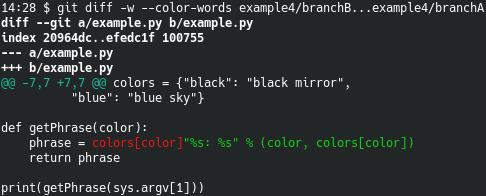
\includegraphics{color_words_02.png}
	\caption{Differences introduced by {\bf branchB}}
	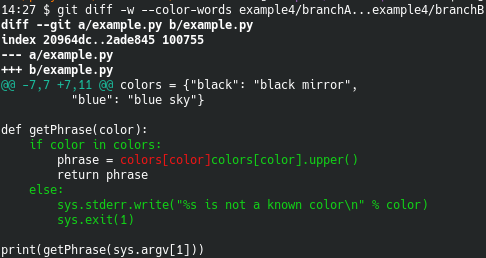
\includegraphics{color_words_01.png}
\end{figure}

When people decide to cut corners and not do a thorough check for the differences they easily end up with changes that are
not copied over from the branches involved (or copying things verbatim deleting other changes) and that is what will
eventually end up exploding later on, sometimes in a {\it BIG... SPECTACULAR... FLASHY WAY.... {\bf in production}}. Certainly not
the best of all places to find out that there was some change that was not carried over when a merge was done a few
months or weeks before.

If code is added on one branch, it should probably end up on the resulting code as well, just like we did with the else section of
code \footnote{I'm not saying copied over verbatim. There might things that have to be adjusted. A variable name was changed? Guess
what you will have to do.}. And deleted code is a special case that has to be analyzed carefully and I will take care of it later on.

\subsection{Exercises}
\subsubsection{Exercise 4 - a git conflict}
From \hyperref[git_repo]{git's repo}, checkout {\bf d9d65e9f6a} and merge {\bf b57e8119e6}.
\footnote{These are the parents of revision {\bf 01f8d78887}}. Solution is \hyperref[exercise_04]{here}.

\subsubsection{Exercise 5 - another git conflict}
From \hyperref[git_repo]{git's repo}, checkout {\bf cf054f817a} and merge {\bf caf388caa1}.
\footnote{These are the parents of revision {\bf 9b6606f43d}}. Solution is \hyperref[exercise_05]{here}.
